% Defence slide 3, panel 2: applying an MPO to an MPS multiplies the bond
% dimension. Squares = operator tensors (as in apply_pair.tex, bulk_extract.tex),
% circles = state tensors (as in motivation_tn.tex). Bond labels are placed
% clear of the tensors: chi between the two rows, D above the operator row.
\documentclass[tikz,border=3pt]{standalone}
\usepackage{amsmath,amssymb}
\definecolor{tnbulk}{RGB}{86,196,229}
\definecolor{tnE}{RGB}{250,200,70}
\definecolor{tnbnd}{RGB}{196,98,22}
\definecolor{ink}{RGB}{35,44,58}
\begin{document}
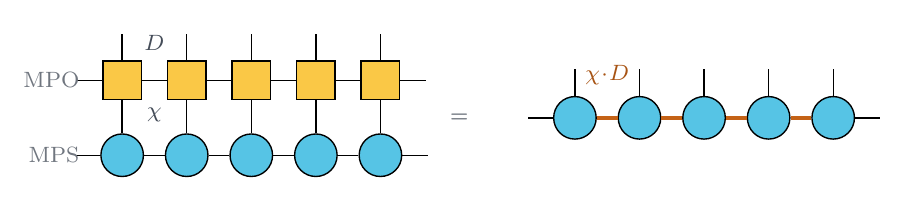
\begin{tikzpicture}[
    W/.style={circle, draw=black, fill=tnbulk, line width=0.5pt,
              minimum size=5.4mm, inner sep=0pt},
    O/.style={rectangle, draw=black, fill=tnE, line width=0.5pt,
              minimum size=4.9mm, inner sep=0pt},
    leg/.style={draw=black, line width=0.5pt},
    lab/.style={font=\footnotesize, color=ink!85},
    tag/.style={font=\footnotesize, color=ink!65}]
  % pinned box: tn_trunc.tex uses the SAME y-limits and puts its chain at the
  % same height, so the two panels align when placed side by side.
  \useasboundingbox (-1.20,-0.34) rectangle (9.70,1.62);
  \def\dx{0.82}
  \def\yo{0.95}      % operator row
  % --- the MPO sitting on the MPS ------------------------------------------
  \foreach \i in {0,...,4} {
    \node[O] (o\i) at ({\i*\dx},\yo) {};
    \node[W] (m\i) at ({\i*\dx},0)   {}; }
  \foreach \i/\j in {0/1,1/2,2/3,3/4} {
    \draw[leg] (o\i.east) -- (o\j.west);
    \draw[leg] (m\i.east) -- (m\j.west); }
  \draw[leg] (o0.west) -- ++(-0.32,0);   \draw[leg] (o4.east) -- ++(0.32,0);
  \draw[leg] (m0.west) -- ++(-0.32,0);   \draw[leg] (m4.east) -- ++(0.32,0);
  \foreach \i in {0,...,4} {
    \draw[leg] (o\i.north) -- ++(0,0.34);
    \draw[leg] (m\i.north) -- (o\i.south); }
  \node[tag, anchor=east] at (-0.42,\yo) {MPO};
  \node[tag, anchor=east] at (-0.42,0)   {MPS};
  \node[lab, anchor=south] at ({0.5*\dx},{\yo+0.26}) {$D$};
  \node[lab, anchor=south] at ({0.5*\dx},0.30)       {$\chi$};
  % --- equals one chain with a fatter bond ----------------------------------
  \node[lab] at ({4*\dx+1.00},{0.5*\yo}) {$=$};
  \foreach \i in {0,...,4} { \node[W] (n\i) at ({5.75+\i*\dx},{0.5*\yo}) {}; }
  \foreach \i/\j in {0/1,1/2,2/3,3/4} {
    \draw[leg, tnbnd, line width=1.3pt] (n\i.east) -- (n\j.west); }
  \draw[leg] (n0.west) -- ++(-0.32,0);  \draw[leg] (n4.east) -- ++(0.32,0);
  \foreach \i in {0,...,4} { \draw[leg] (n\i.north) -- ++(0,0.34); }
  \node[lab, anchor=south, color=tnbnd!85!black]
    at ({5.75+0.5*\dx},{0.5*\yo+0.30}) {$\chi\!\cdot\! D$};
\end{tikzpicture}
\end{document}
